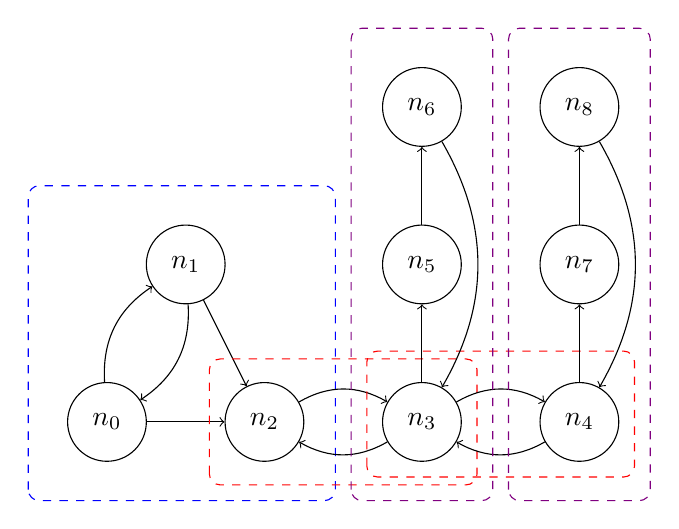
\begin{tikzpicture}[neuron/.style={circle, minimum size=1cm, draw=black!100}]
    \draw[rounded corners, blue, dashed] (0, 0) rectangle (3.9, 4);
    
    \node[neuron] (h-1) at (2, 3) {$n_1$};
    \node[neuron] (h-0) at (1, 1) {$n_0$};
    \node[neuron] (h-2) at (3, 1) {$n_2$};
    
    \draw[->] (h-0) edge [bend left] (h-1);
    \draw[->] (h-1) edge [bend left] (h-0);
    \draw[->] (h-1) -- (h-2);
    \draw[->] (h-0) -- (h-2);
    

    \draw[rounded corners, red, dashed] (2.3, 0.2) rectangle (5.7, 1.8);
    
    \node[neuron] (h-3) at (5, 1) {$n_3$};
    
    \draw[->] (h-2) edge [bend left] (h-3);
    \draw[->] (h-3) edge [bend left] (h-2);
    

    \draw[rounded corners, red, dashed] (4.3, 0.3) rectangle (7.7, 1.9);
    
    \node[neuron] (h-4) at (7, 1) {$n_4$};
    
    \draw[->] (h-3) edge [bend left] (h-4);
    \draw[->] (h-4) edge [bend left] (h-3);
    

    \draw[rounded corners, violet, dashed] (4.1, 0) rectangle (5.9, 6);

    \node[neuron] (h-5) at (5, 3) {$n_5$};
    \node[neuron] (h-6) at (5, 5) {$n_6$};

    \draw[->] (h-3) -- (h-5);
    \draw[->] (h-5) -- (h-6);
    \draw[->] (h-6) edge [bend left] (h-3);


    \draw[rounded corners, violet, dashed] (6.1, 0) rectangle (7.9, 6);

    \node[neuron] (h-7) at (7, 3) {$n_7$};
    \node[neuron] (h-8) at (7, 5) {$n_8$};
    
    \draw[->] (h-4) -- (h-7);
    \draw[->] (h-7) -- (h-8);
    \draw[->] (h-8) edge [bend left] (h-4);
\end{tikzpicture}
